\chapter{Introduction}
\label{chapter:introduction}

\begin{quote}
{\itshape
This chapter motivates the need of creating better malware ground truth.

The first section analyzes the state of mobile security for Android application.

The second section discusses challenges for the Android security community.

The third section summarizes the research contributions of this dissertation.
}
\end{quote}

\localtableofcontents{}

\section{Mobile security in the real world}
\subsection{Mobile security and innovation}
\subsubsection{Growths of mobile ecosystems}

\begin{figure}[!ht]
        \centering
	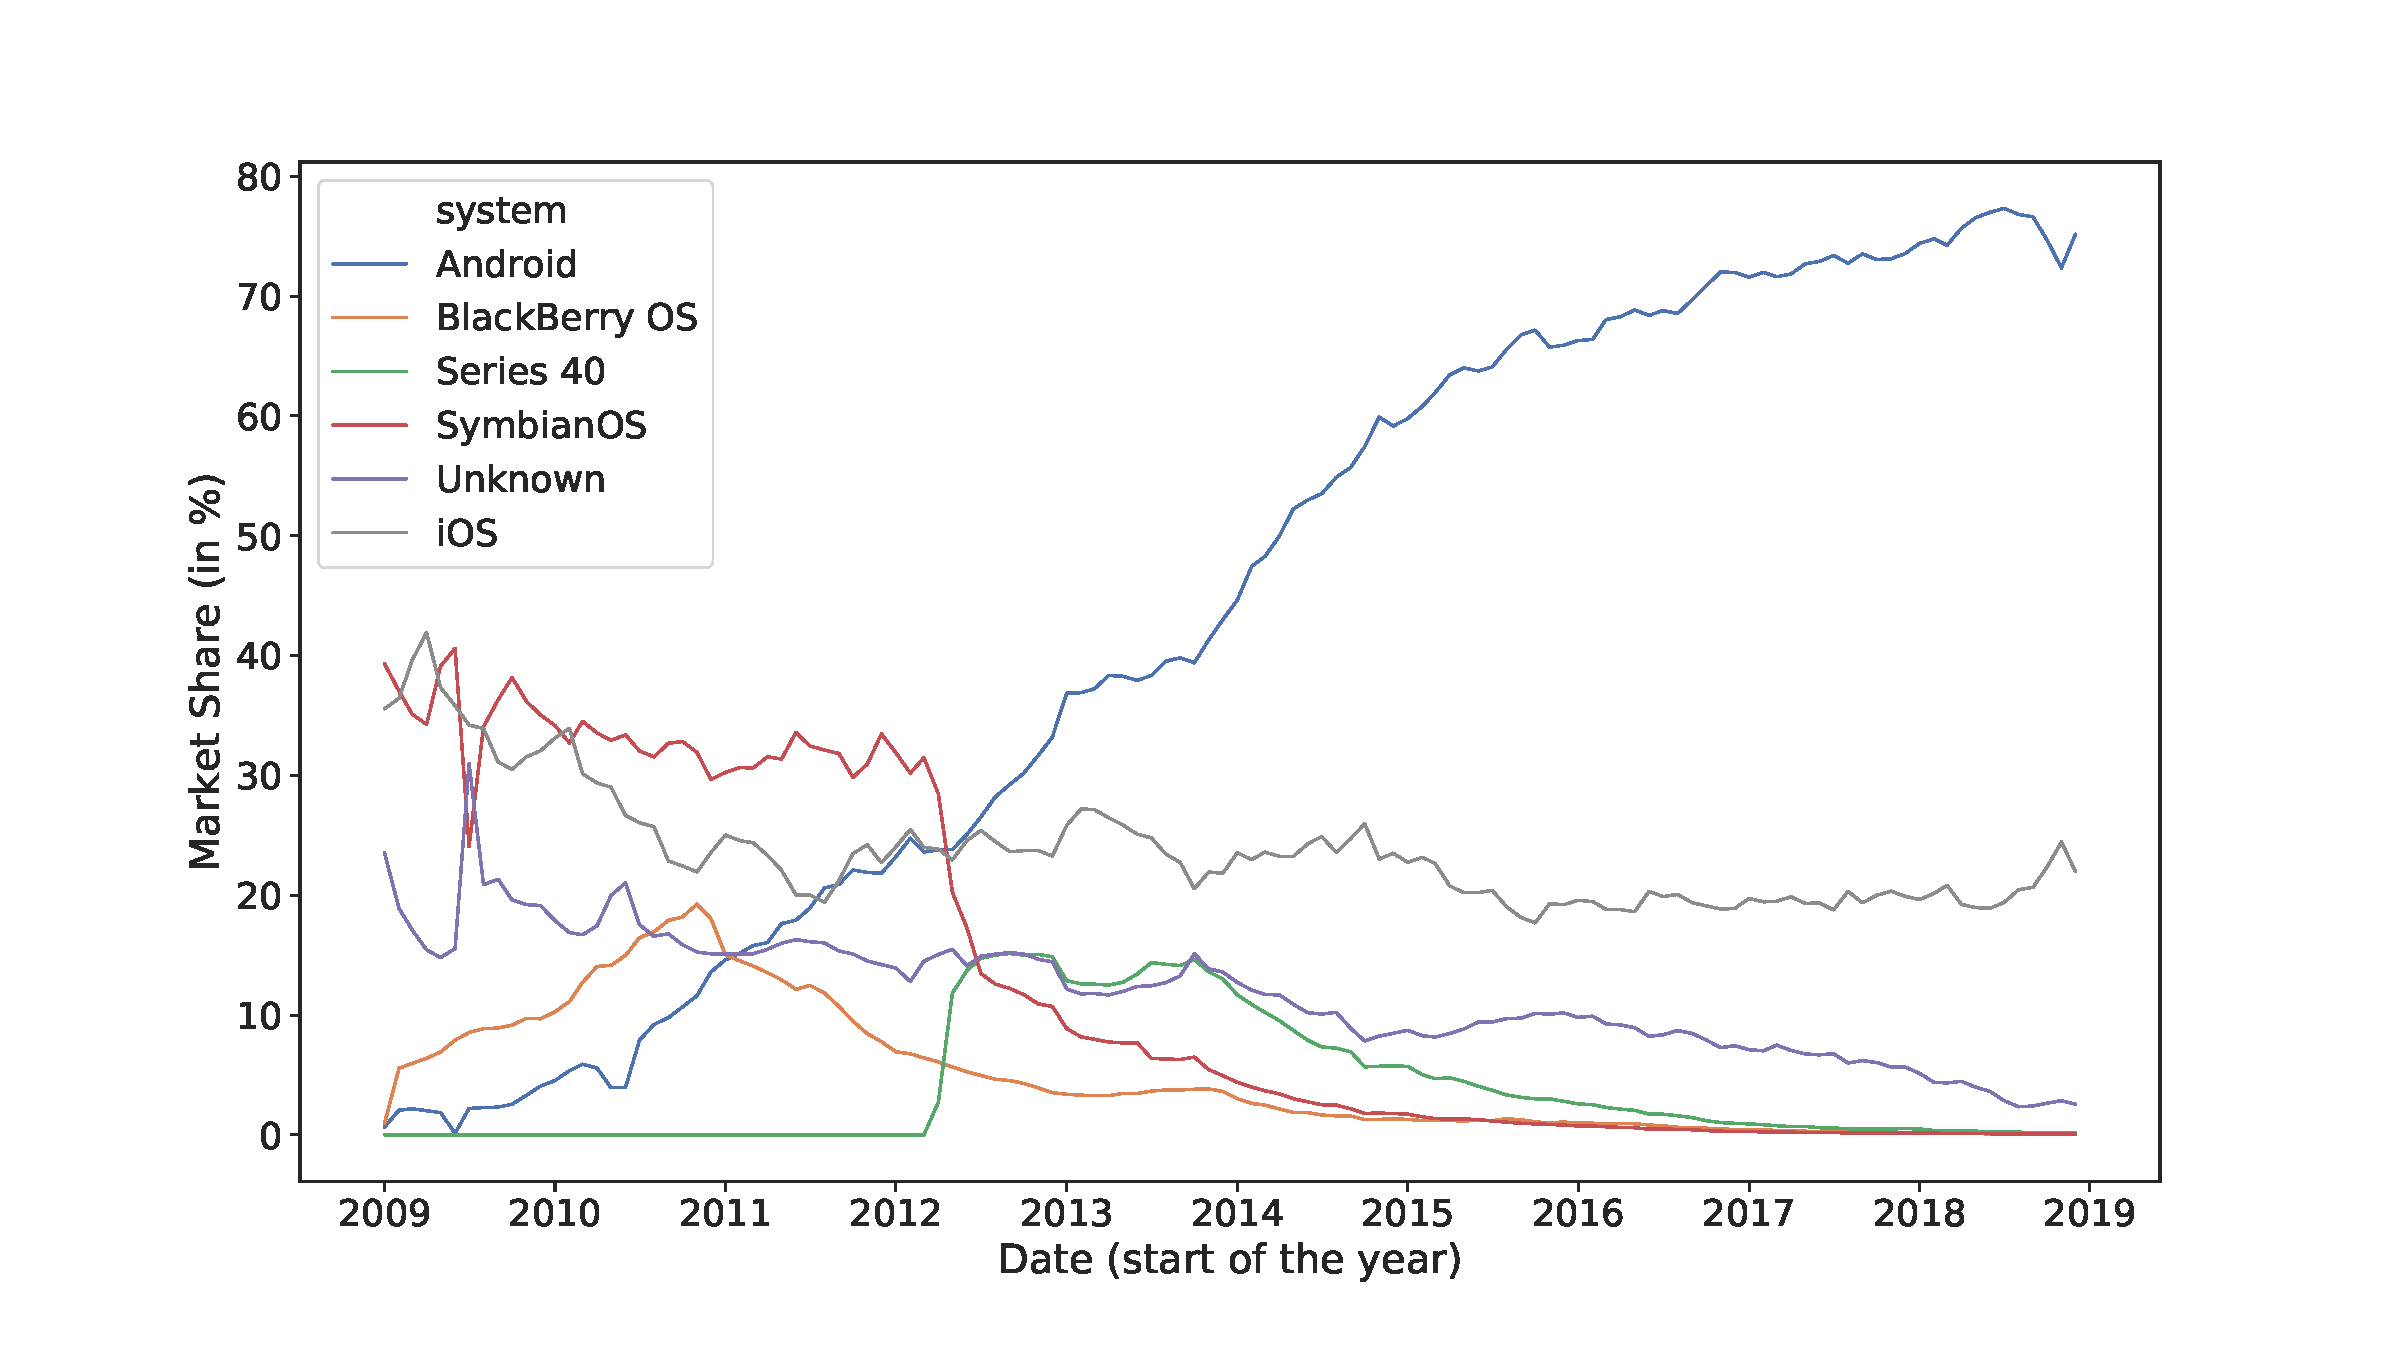
\includegraphics[width=\linewidth]{figures/introduction/marketshare.pdf}
        \caption[Market shares of mobile operating systems]{Market shares of mobile operating systems, StatCounter~\cite{statcounter_mobile_2019}}
	\label{figure:introduction:marketshare}
\end{figure}

The mobile industry is a sector in constant evolution, thanks to the adoption of innovative technologies such as Android.
In 2018, Google LLC identified at least 2 billion active devices powered by a version of Android~\cite{google_android_2018}.
Moreover, Figure~\ref{figure:introduction:marketshare} shows that Android became the leading mobile operating system in 2012, with a global market share superior to 70\% in 2019.

\begin{figure}[!ht]
        \centering
	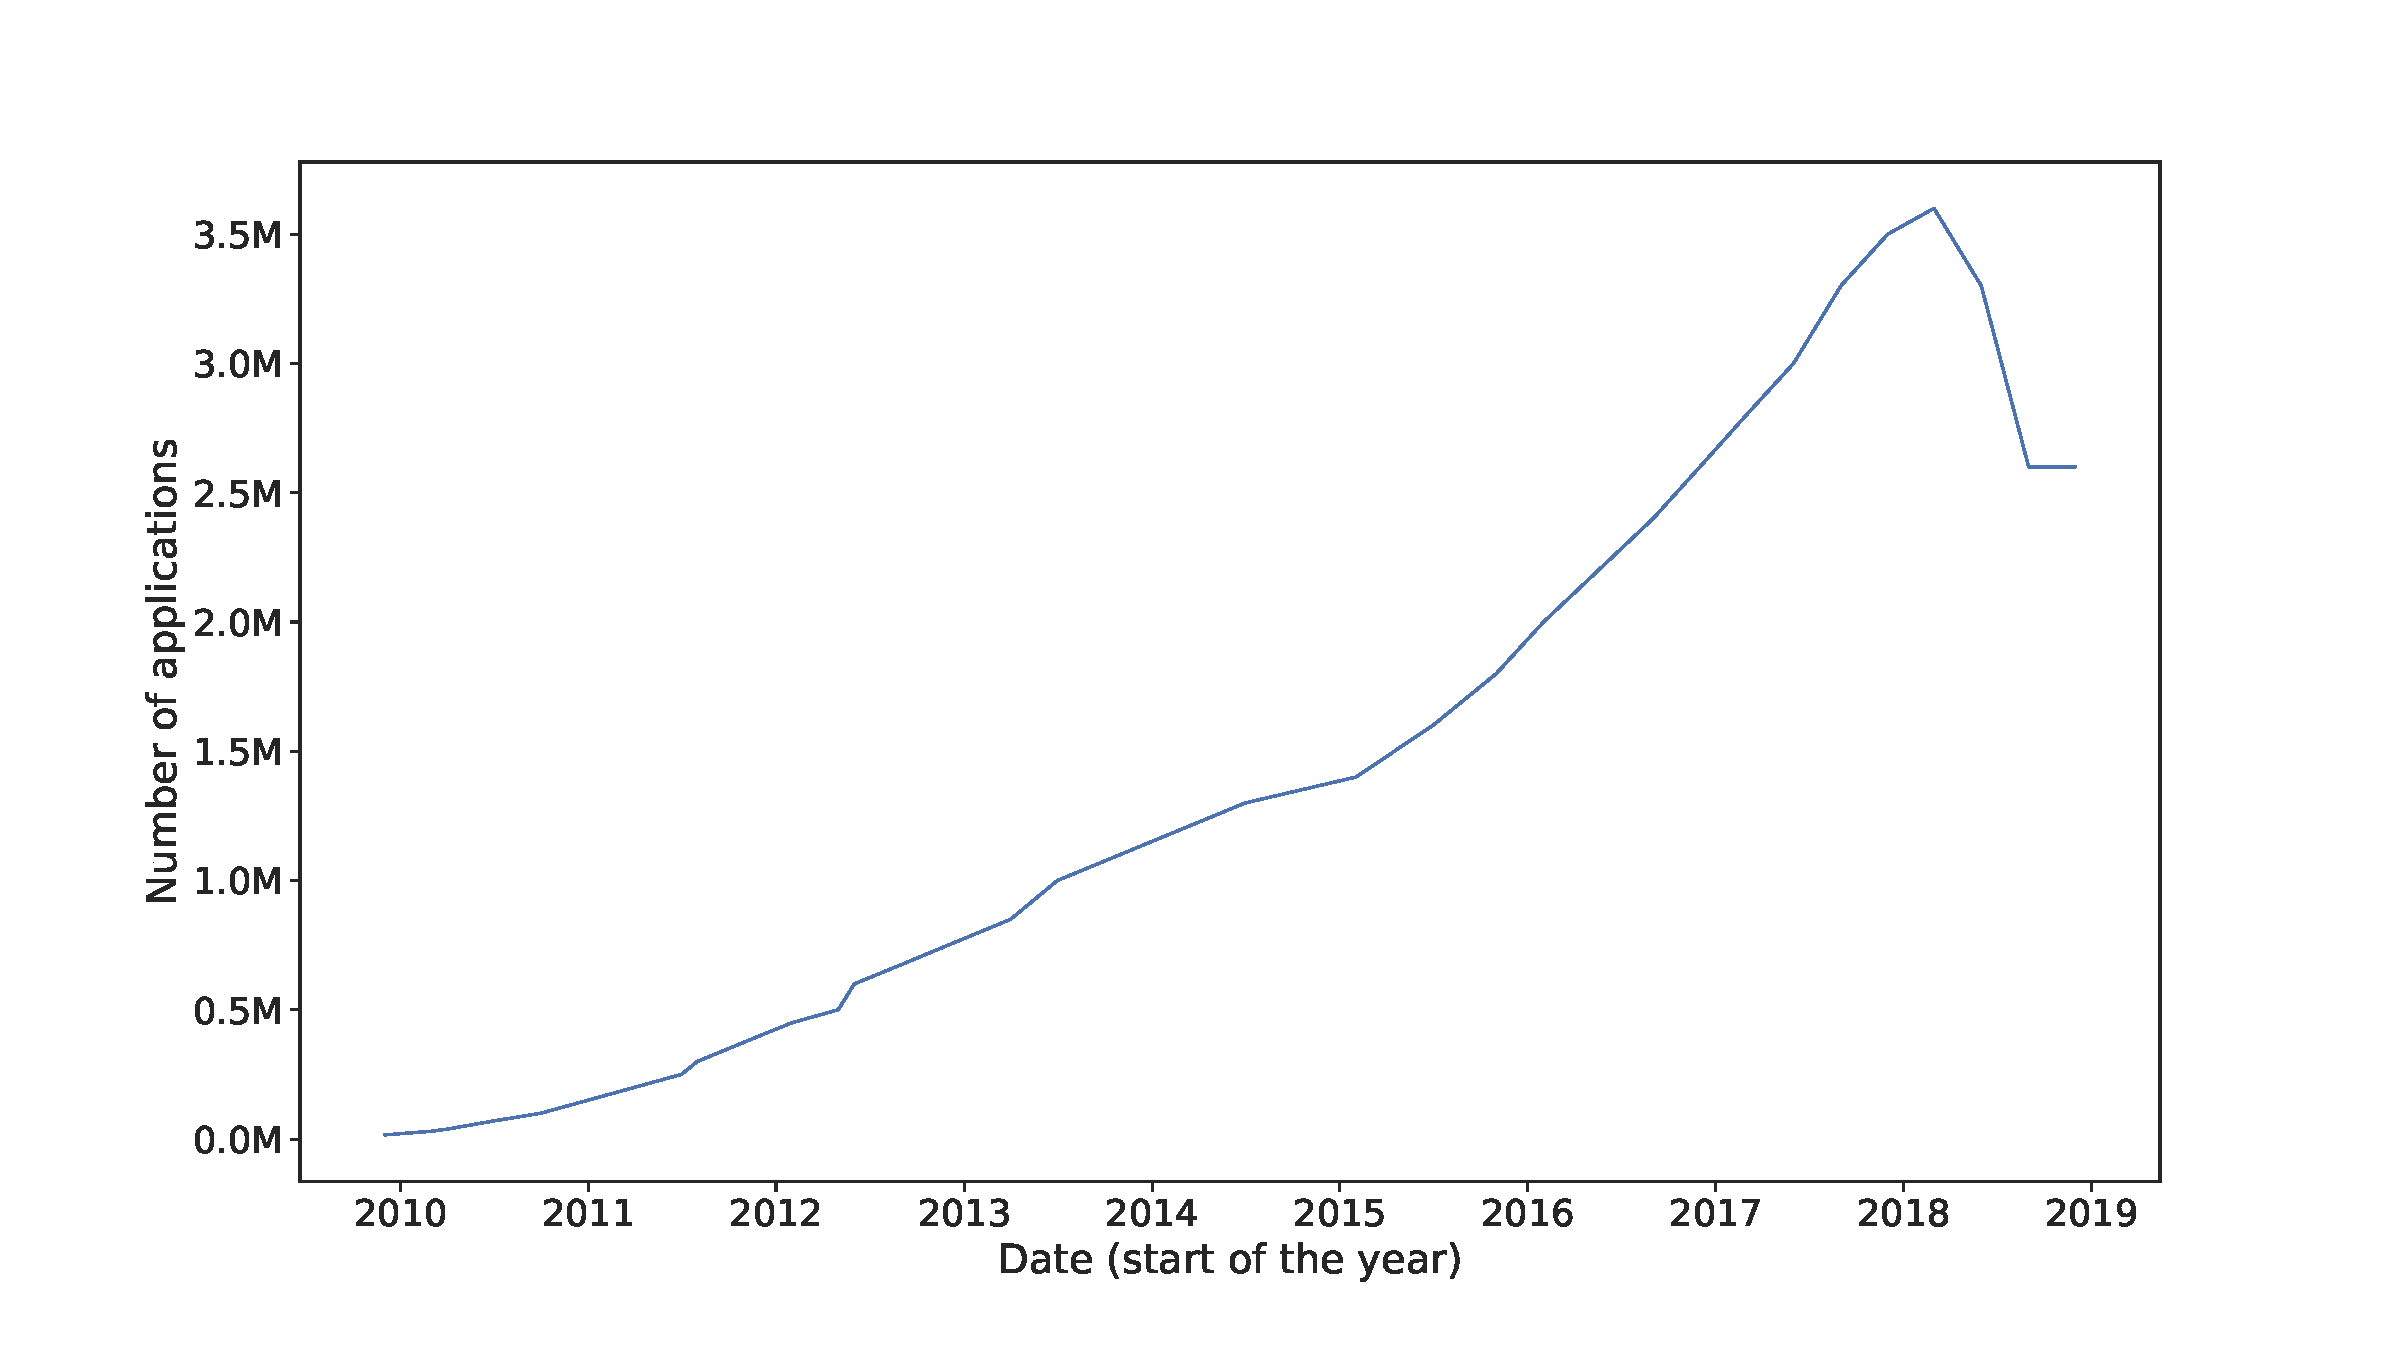
\includegraphics[width=\linewidth]{figures/introduction/applications.pdf}
        \caption[Number of applications available on Google Play]{Number of applications available on Google Play, Statista~\cite{statista_number_2019}}
	\label{figure:introduction:applications}
\end{figure}

The success of Android can be explained by the development of the supply and demand for mobile services.
On the one hand, mobile users adopt Android solutions for managing everything that relates to their personal and professional life, ranging from social networking to financial investments.
On the other hand, Android developers meet the demand of mobile users with a growing catalog of applications distributed on digital marketplaces such as Google Play~\cite{google_google_2019}.
Figure~\ref{figure:introduction:applications} illustrates the growing number of applications released on Google Play from 2009 to 2018.
We can observe that 3.5 million applications were available on the platform in 2018~\cite{statista_number_2019}.
In this context of social and economic growth, the task of protecting mobile devices has become more important than ever to support the expansion of mobile ecosystems.
\subsubsection{Implications for mobile security}
We can define mobile security as the perception that nothing wrong can happen to mobile users, mobile hardware, or the information stored on mobile devices.
It is a fundamental right that every mobile user should be entitled to, even for immaterial assets such as personal information.

\begin{figure}[!ht]
        \centering
	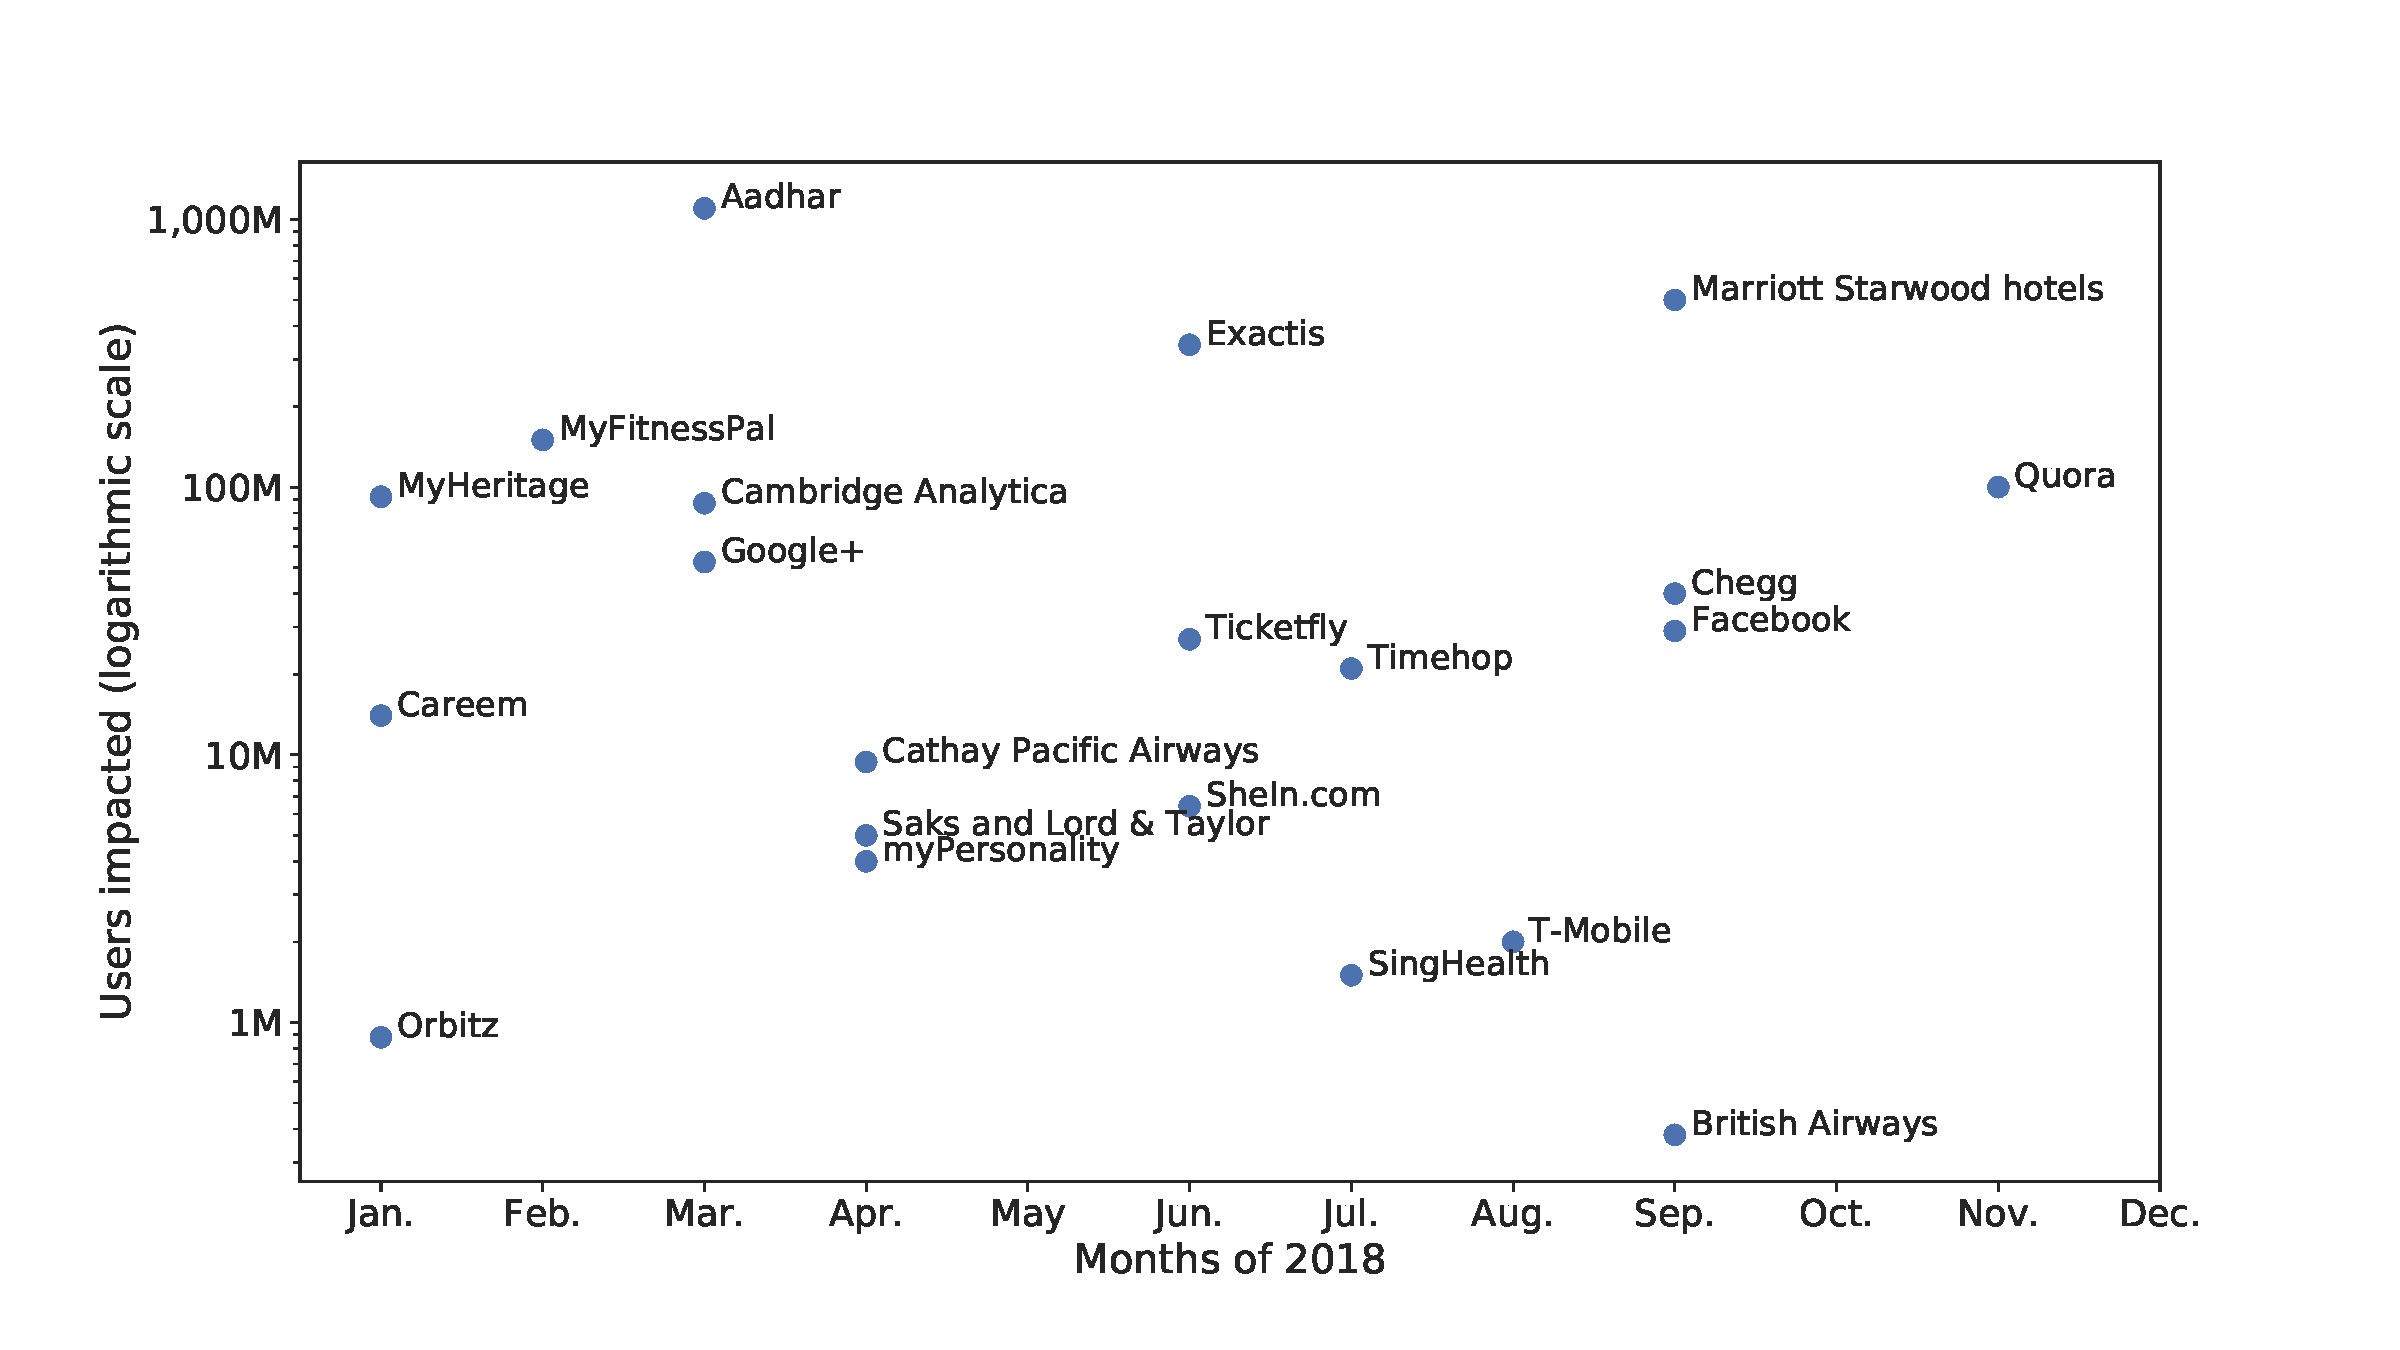
\includegraphics[width=\linewidth]{figures/introduction/breaches.pdf}
        \caption[The 21 scariest data breaches of 2018]{The 21 scariest data breaches of 2018, Business Insider~\cite{leskin_21_2018}}
	\label{figure:introduction:breaches}
\end{figure}

However, not a single month goes by without a global security breach or a privacy issue that impacts thousands of users~\cite{leskin_21_2018}.
Figure~\ref{figure:introduction:breaches} shows that the top 21 data breaches of 2018 impacted between 200,000 and 1 billion users each.
We can conclude from these observations that the global lack of security continues to have real consequences on people life, which may deter mobile users from trusting digital marketplaces.
\subsection{Mobile security as an arms race}
\subsubsection{Profiles of security attackers}
Mobile security involves two main actors: an attacker whose goal is to harm the security of mobile users, and a defender that must guarantee an acceptable level of security in the presence of attackers.
Attackers can be criminals, activists, state-affiliated employees, or other types of associations.
Figure~\ref{figure:introduction:actors} shows the distribution of attackers' origin and motive identified in Verizon data break report~\cite{verizon_2018_2019}.
We can observe that while the origin of 63\% attacker is unknown, their actions are motivated 43\% of the time by financial gains.

\begin{figure}[!ht]
        \centering
	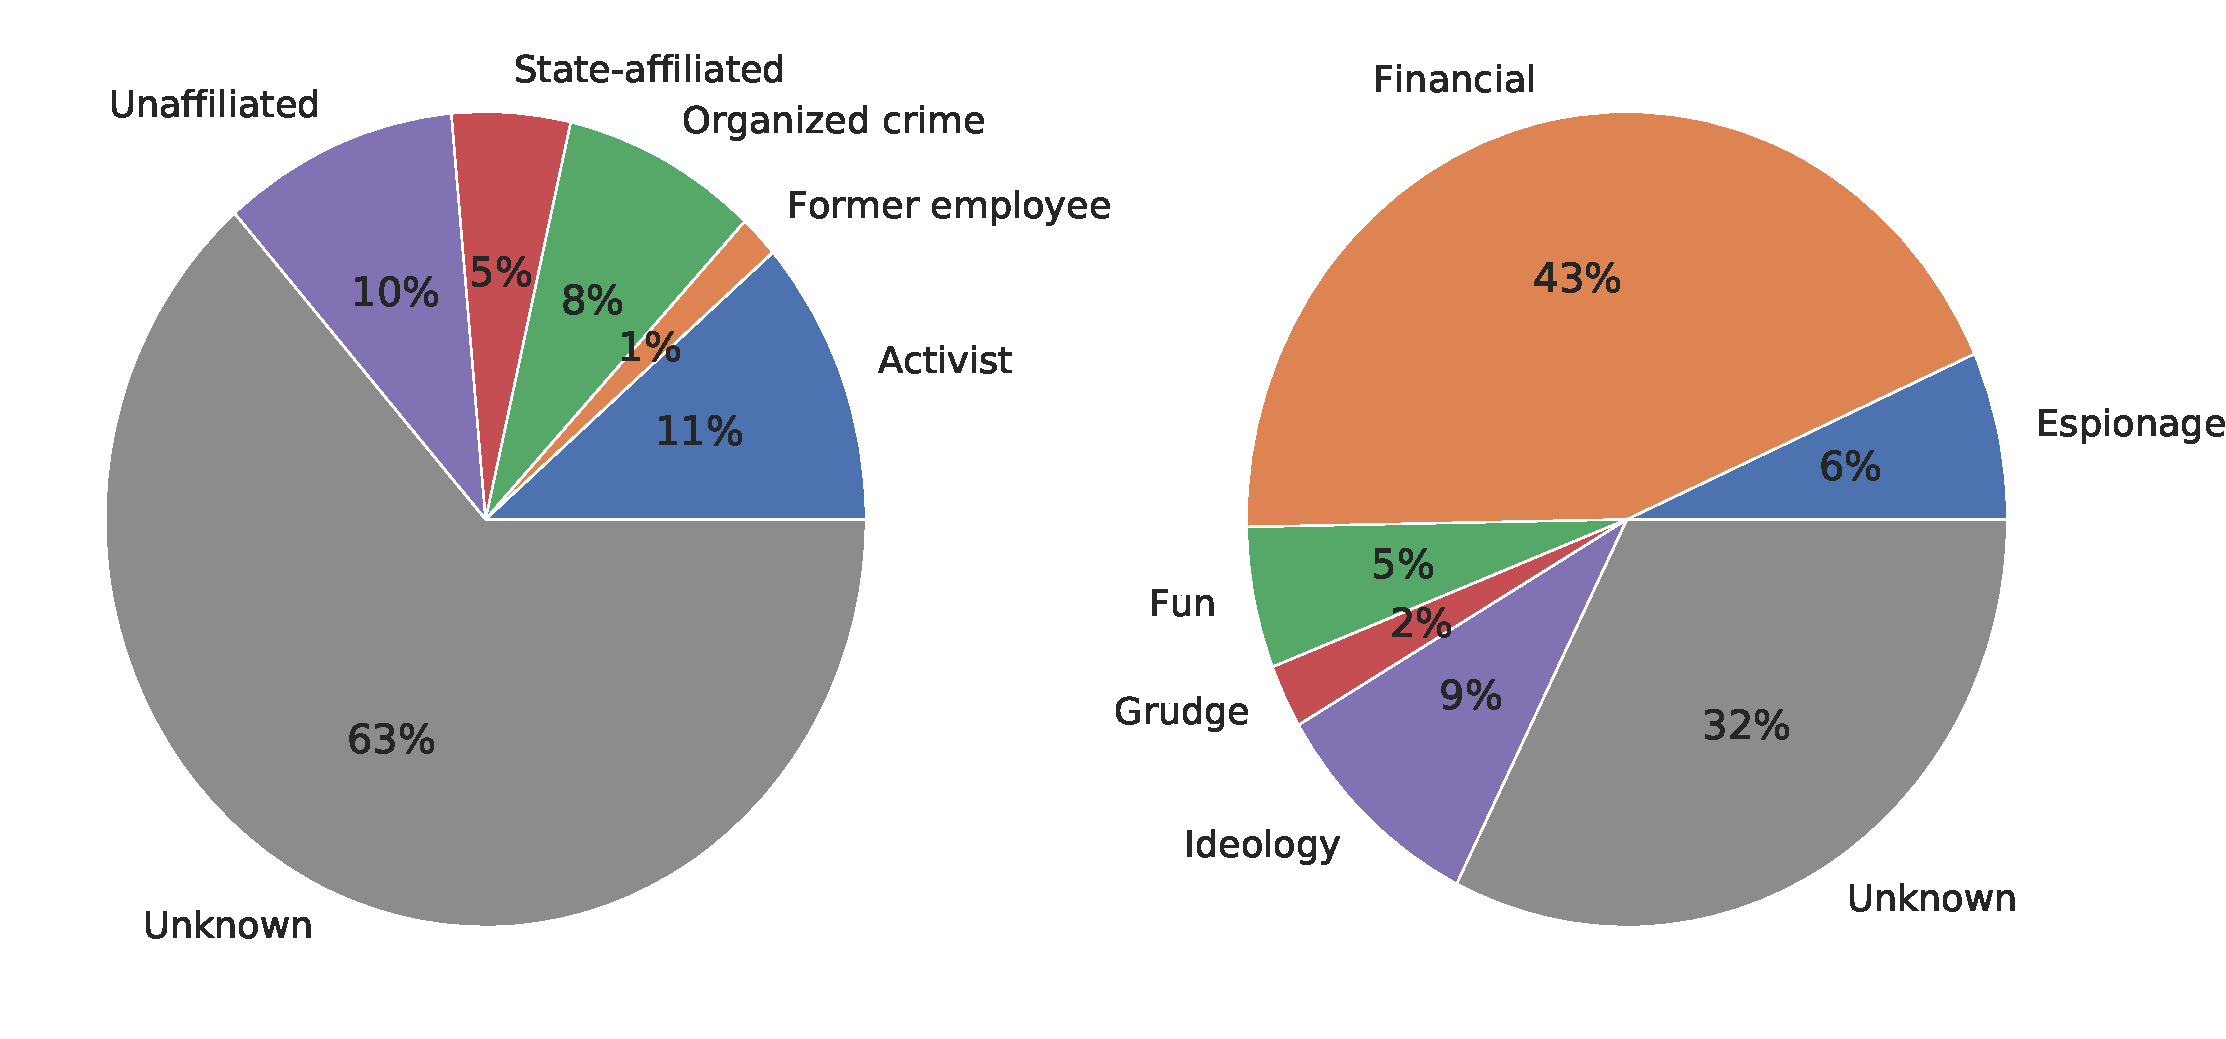
\includegraphics[width=\linewidth]{figures/introduction/actors.pdf}
        \caption[Profile of security attackers by origin and motive]{Profile of security attackers by origin (left) and motive (right), Verizon VCDB~\cite{verizon_2018_2019}}
	\label{figure:introduction:actors}
\end{figure}

Furthermore, we can note that attackers tend to target infrastructures with the weakest security measures in place~\cite{verizon_2018_2019}.
This model is similar to a military arms race, where every technological edge can shift the balance of power between belligerents.
Compared to other sectors, it is crucial to highlight that mobile security requires constant technological improvements to address the ever-changing risks associated with this landscape.
\subsubsection{Efforts of the security community}
To undertake the threats posed by attackers, the security community engaged tremendous effort in the development of better threat mitigation techniques.
In 2018, Google announced that the annual probability for a user to download malware from Google Play was 0.02\%, which is according to the report `less likely than the odds of an asteroid hitting the earth`~\cite{google_android_2018}.

To contrast this figure, the Sophos threat report of 2019 mentions that the release of malware targeting mobile and IoT devices is not slowing down~\cite{sophos_sophoslabs_2019}.
The report points out unusual malicious campaigns, including crypto-miner code in games, advertising click fraud, and supply chain compromise that bypassed the security of Google Play.
Since no trusted third party can firmly confirm or infirm the current state of mobile security, we must consider a conservative scenario where the mobile industry continues to face security challenges.
\subsection{Mobile security for Android applications}
\subsubsection{The principle of least privilege}
The security model of Android applications rests upon the well-known principle of least privilege~\cite{google_permissions_2019}.
This principle states that an application should always operate with the least amount of privilege to perform its task.
For instance, a banking application might request Internet access to manage online accounts, but requesting access to contact information would be suspicious behavior for this category of application.

The decision to allow or deny a permission to an application currently relies on mobile users.
This principle is then enforced by the Android operating system, which acts as a gatekeeper to access the personal information of mobile users.
For instance, Figure~\ref{figure:introduction:permissions} shows a permission dialog that requests access to contact information.
If the user grants the permission, the application can keep access to contact information as long as the permission is not revoked.
Otherwise, the application will keep asking for the same permission to enable one of its features.
At any point during the authorization process, an Android user can block the application from asking the same request over and over again.

\begin{figure}[!ht]
        \centering
	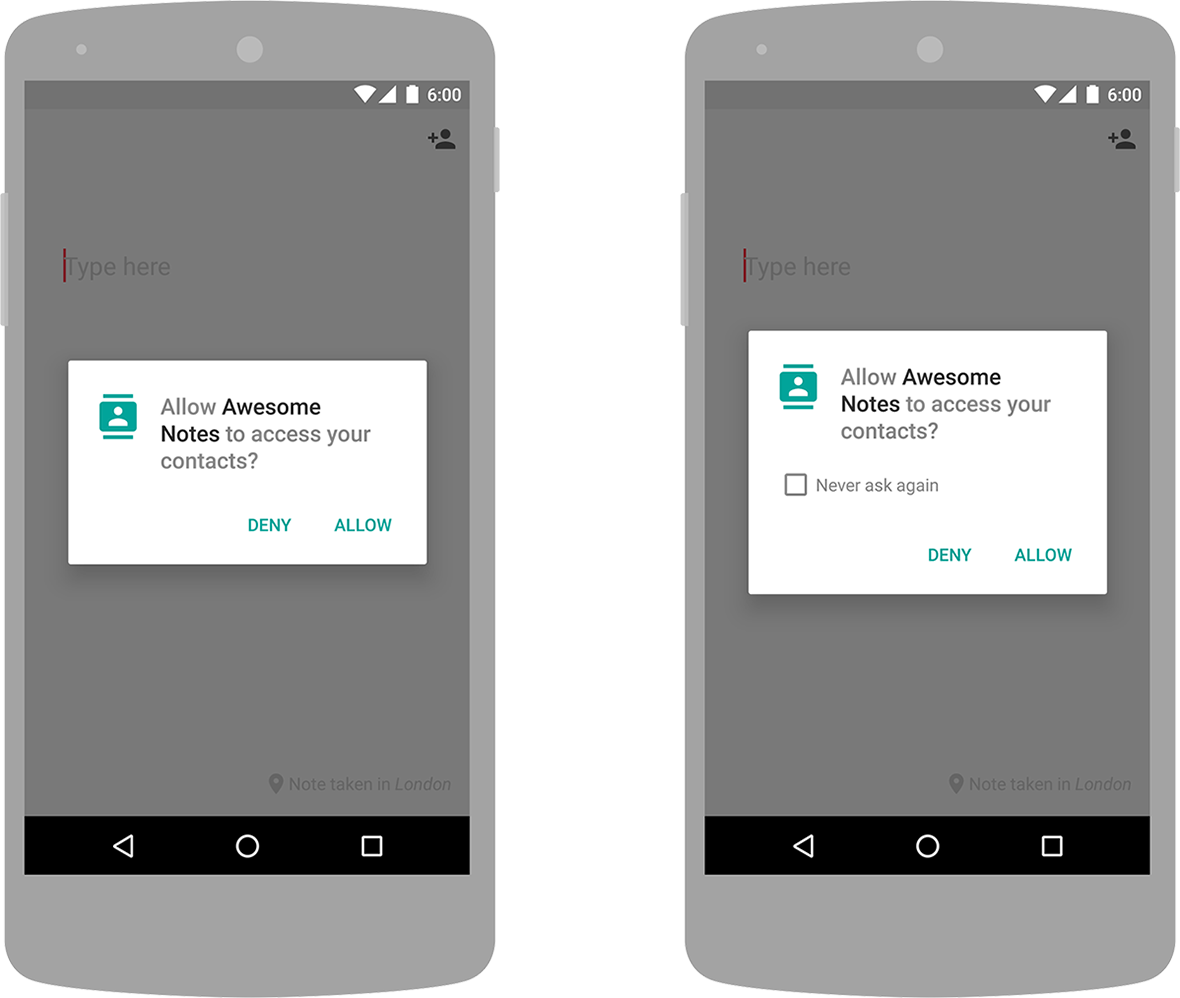
\includegraphics[width=0.65\linewidth]{figures/introduction/permissions.png}
	\caption{Permission dialog to let an application access user contacts}
	\label{figure:introduction:permissions}
\end{figure}

In theory, the security model of Android applications is supposed to provide much more security and flexibility than for regular desktop applications~\cite{google_permissions_2019}.
On the one hand, end users are always in control of the operations that an application can perform on their device.
On the other hand, the operating system can take into account user inputs to better decide on how to handle application permissions.

However, this model is not sufficient to deny the exploitation of user information in practice~\cite{google_android_2018}.
First, the implementation of the principle of least privilege is not granular enough to protect against a specific type of misuse or scam (e.g.,\ which information are sent over the Internet).
Second, end users might not have enough information to make an informed decision about the level of permission to grant to an application.
Finally, end users do not have the knowledge nor the expertise to understand the implication of their choices fully.

For these reasons, the security of Android systems cannot depend solely on the implementation of the principle of least privilege.
Both human and system experts must evaluate the characteristics of Android applications to guide end users and remove lurking threats from Android marketplaces.
\subsubsection{Example of an Android malware}
To illustrate the threats that target the Android ecosystem, let us consider a malware analyzed by Upstream Systems in January 2019~\cite{upstream_systems_secure-d_2019}.
The company identified a weather forecast application developed by a Chinese company.
At the time of the investigation, the application was pre-installed on Alcatel Android smartphones, such as the Pixi 4 and A3 Max models.

Upstream Systems identified that the weather application leaks user information such as the geographic locations, email addresses, smartphone identifiers (IMEIs), and send them back to a server in China~\cite{upstream_systems_secure-d_2019}.
Moreover, the application uses a background task to subscribe users to unwanted paid services for an estimated earning of \$ 1.5 million.
The application was available on Google Play during the investigation by Upstream Systems, with more than 10 million installs and a user rating of 4.4 out of 5 when they disclosed their analysis.
Figure~\ref{figure:introduction:weather} displays a screenshot of the application as it could be found on Google Play, under the name TCL Weather.

\begin{figure}[!ht]
        \centering
	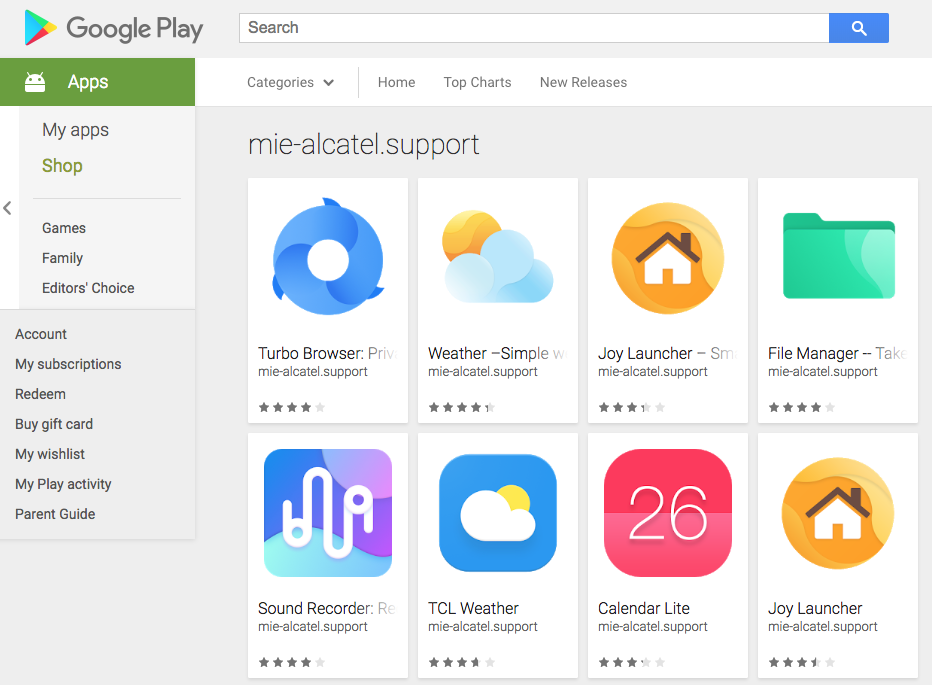
\includegraphics[width=0.75\linewidth]{figures/introduction/weather.png}
	\caption{Android applications of 'mie-alcatel.support' on Google Play}
	\label{figure:introduction:weather}
\end{figure}

The investigation of Upstream Systems unveiled that the application was requesting invasive permissions.
Table~\ref{table:introduction:weather} enumerates the permissions and the personal information requested by the application.
With these accesses, the application could click on ads banner without the consent of the device owner.
Upstream Systems also found that the application could issue more than 250 transaction requests per month, leading to unwanted charges, additional network consumption, and device overheating.

Following the publication of Upstream Services findings, the application was removed from Google Play on the 5th of January 2019~\cite{upstream_systems_secure-d_2019}.
Nevertheless, the reaction of Google Play came too late, as more than 10 million users already installed the application on their device.
This story illustrates that the lack of security on mobile devices is real and can impact a large population of users across the world.

\begin{table}[!ht]
    \label{table:introduction:weather}
    \caption{Permissions requested by the application 'com.tct.weather'}
    \begin{tabularx}{\textwidth}{|c|X|}
    \hline
    Permission & What it allows \\ \hline
    CHANGE\_WIFI\_STATE & Allows the application to change the state of the wi-fi network. \\ \hline
    MOUNT\_UNMOUNT\_FILESYSTEMS & Allows mounting and unmounting of file systems (i.e.,\ external SD cards). Android documentation says the permission is NOT intended for third-party applications \\ \hline
    READ\_PHONE\_STATE & Allows read-only access to phone state, including the phone number of the device, current cellular network information, the status of any ongoing calls, and a list of any PhoneAccounts registered on the device. Documentation says that this permission is DANGEROUS \\ \hline
        WRITE\_EXTERNAL\_STORAGE & Allows reading and writing of the external storage. This is dangerous (as the application can have access to other user files and third-party logs, system logs). This means that the application can read/write everything it wants and the read data might be sent to the server. \\ \hline
    ACCESS\_KEYGUARD\_SECURE\_STORAGE & This permission was removed in the OS since 4.4 (KitKat). However, for devices that are below that version, this permission can control a flaw in the OS to lock and unlock the device at any time (like pressing the power button and unlocking the phone) \\ \hline
    READ\_LOGS & Allows an application to read the low-level system log files. Not for use by third-party applications, because Log entries can contain the user’s private information. \\ \hline
    SET\_DEBUG\_APP & Configure an application for debugging. Not for use by third-party applications. \\
    \hline
    \end{tabularx}
\end{table}


\section{Android security challenges}
\subsection{Definition of Android malware}
\subsubsection{Importance of malware definition}
While we could state that a malware is a piece of software that causes harm to end users~\cite{oxford_dictionnary_malware_2019}, this definition on its own is not sufficient at a technical level to detect malicious applications.

On the one hand, maliciousness is a notion more relative than absolute.
For instance, let us consider two Android applications that upload documents on a remote server.
Depending on the appreciation of each user, one application could be considered malicious while the other would not.
As Figure~\ref{figure:introduction:definition} illustrates, the decision to classify an application as malicious relies on an implicit contract between end users, developers, and digital marketplaces.
If an end user is not informed about the intents of the developer, or if the platform imposes restrictions that are not met, then the contract is breached, and the application should be considered as potentially malicious by at least one of the parties involved.
The goal of security experts in this context is to report which application components are unwanted to prevent their installation on mobile devices~\cite{google_android_2018}.

On the other hand, the detection of malicious applications can be automated by a computer system if and only if the specification for this task is explicit and unambiguous.
Since computers are not aware of the concept of harm and maliciousness, computer systems require a formal definition to return the security status of an application.
In a landscape where Android malware is on the rise, the power of computer systems has to be leveraged to automate the analysis of Android applications and detect potential malware.

\begin{figure}[!ht]
	\centering
	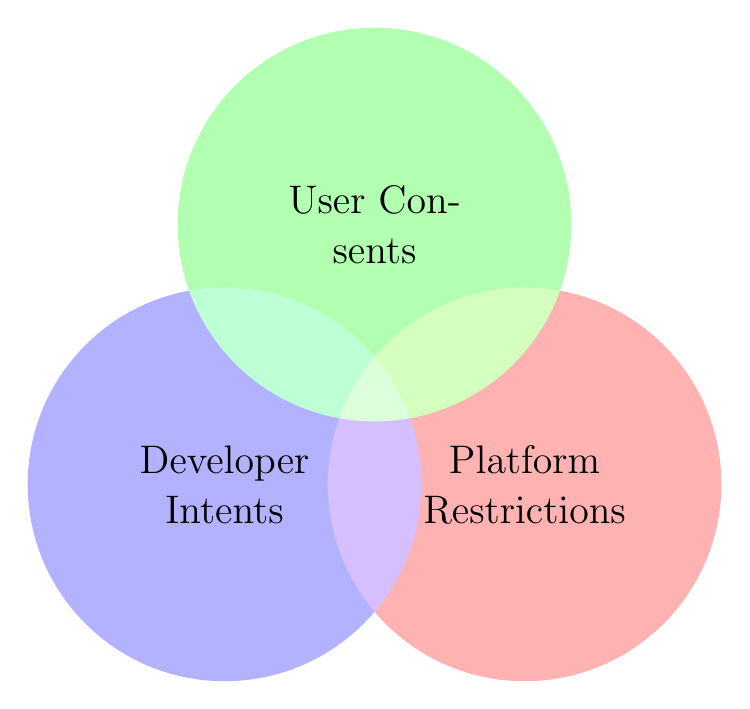
\begin{tikzpicture}
    \begin{scope}[blend group = soft light]
        \fill[green!30!white] (90:2.2) circle (2.5);
        \fill[blue!30!white] (210:2.2) circle (2.5);
        \fill[red!30!white] (330:2.2) circle (2.5);
    \end{scope}
    \node[text width=3cm, align=center, font=\Large] at (90:2.2) {User Consents};
    \node[text width=3cm, align=center, font=\Large] at (210:2.2) {Developer Intents};
    \node[text width=3cm, align=center, font=\Large] at (330:2.2) {Platform Restrictions};
\end{tikzpicture}

	\caption{The definition of malware at the intersection of 3 other notions}
	\label{figure:introduction:definition}
\end{figure}

Hence, our ability to prevent the propagation of malware depends heavily on our capacity to characterize Android applications.
Without a proper characterization, security experts lack the requirements to properly define malicious behaviors and automate their detection by computer systems in the large.
In this regard, one of the key challenges for the security community is to provide a thorough and accurate report on the components contained in Android applications and explain how these components are associated with malicious behaviors.
\subsubsection{Solving the lack of malware definition}
In the absence of a formal definition, digital marketplaces must rely on human inputs to assess the dangerousness of Android applications.
To illustrate this process, Figure~\ref{figure:introduction:antivirus} shows the analysis of Android applications from the viewpoint of a security organization.
At the beginning of the process, samples are collected directly from the Internet or from online user submissions.
Security experts can then analyze the application components and isolates which one are involved in the expression of malicious behaviors.
The expert can later label the applications as either benign or malicious, and provide some generic rules to classify similar applications with the same tag.
In this process, we notice that human expertise is essential to detect Android malware, as experts provide valuable results and knowledge that can be reused by computer systems and other analysts.

\begin{figure}[!ht]
	\centering
	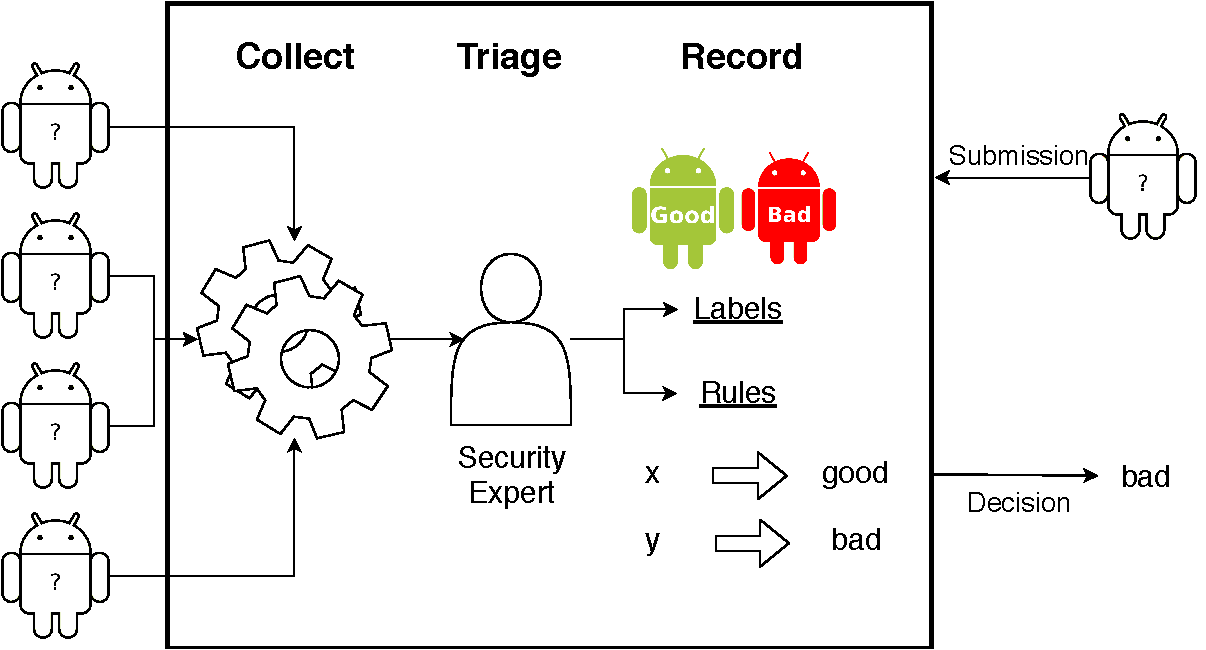
\includegraphics[width=\linewidth]{figures/introduction/antivirus.pdf}
	\caption{Initial analysis and vetting process of Android applications}
	\label{figure:introduction:antivirus}
\end{figure}

While most security organizations have structured themselves around this process, no single organization can cover the current demand for malware analysis on its own.
Besides, few security organizations share the knowledge they gathered about malware publicly or with other organizations, as this knowledge gives them an edge over their competitors.
Due to this lack of communication, the security community can only access small tokens of information from security organizations.
This information is often sparse, unstructured, and lacks the level of details required to understand the relationship between application components and malicious behaviors.
On Figure~\ref{figure:introduction:symantec}, we display a screenshot containing the information shared by Symantec about the malware family Android.Kuguo.
While the article describes the malicious behaviors and the risks associated with this malware family, the company fails to mention both the malicious components involved and the steps to reproduce the analysis.

\begin{figure}[!ht]
	\centering
	\fbox{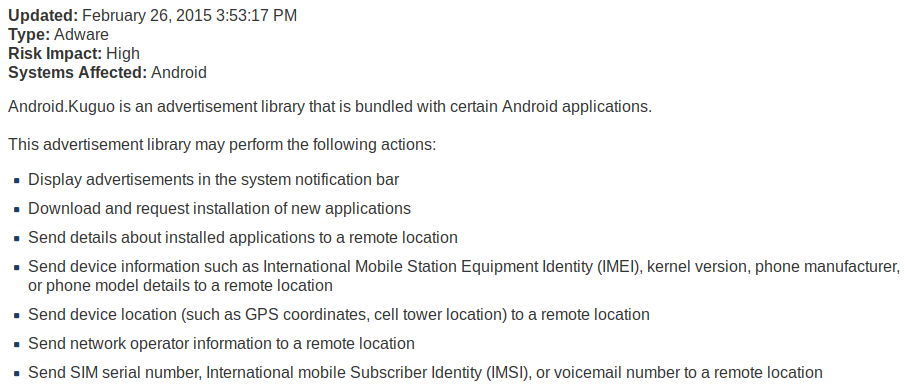
\includegraphics[width=\linewidth]{figures/introduction/symantec.png}}
        \caption[Information about 'Android.Kuguo' from Symantec website]{Information about 'Android.Kuguo' from Symantec website~\cite{symantec_android.kuguo_2019}}
	\label{figure:introduction:symantec}
\end{figure}

To provide a definitive answer to the lack of malware definition, the security community must not only report the effects caused by malicious applications, but also the causes and the elements related to these effects.
It is only at this condition that the security community can create a reliable infrastructure that supports the growth of the Android ecosystem.
\subsection{Automation of security decisions}
\subsubsection{Shortage of security experts}
Over the years, the security of information systems evolved to become an essential facet of our society.
As more and more people and infrastructure are connected, the risks of security attacks and data leakages are now more important than ever~\cite{leskin_21_2018}.
Governments have strengthened their regulations to enforce a better level of security, while end users are increasingly sensitive to threats posed by unsecured systems.
Unfortunately, the number of individuals capable of handling security events is lagging, leaving many demands for security experts unanswered.

In October 2018, (ICS)$^2$ estimated the future lack of security experts around the globe at nearly 3 million people~\cite{ics2_cybersecurity_2018}.
As we can see on Figure~\ref{figure:introduction:expertise}, the most impacted area will be Asia/Pacific with 2.14 million people, North American with nearly 500,000 people and Europe/Middle East/Africa with 142,000 people.
(ICS)$^2$ also noted that 63\% of participating organizations are suffering a shortage of security experts right now and that 60\% of the respondent are at moderate or extreme risk of security attacks as a result of this shortage.

\begin{figure}[!ht]
        \centering
	\fbox{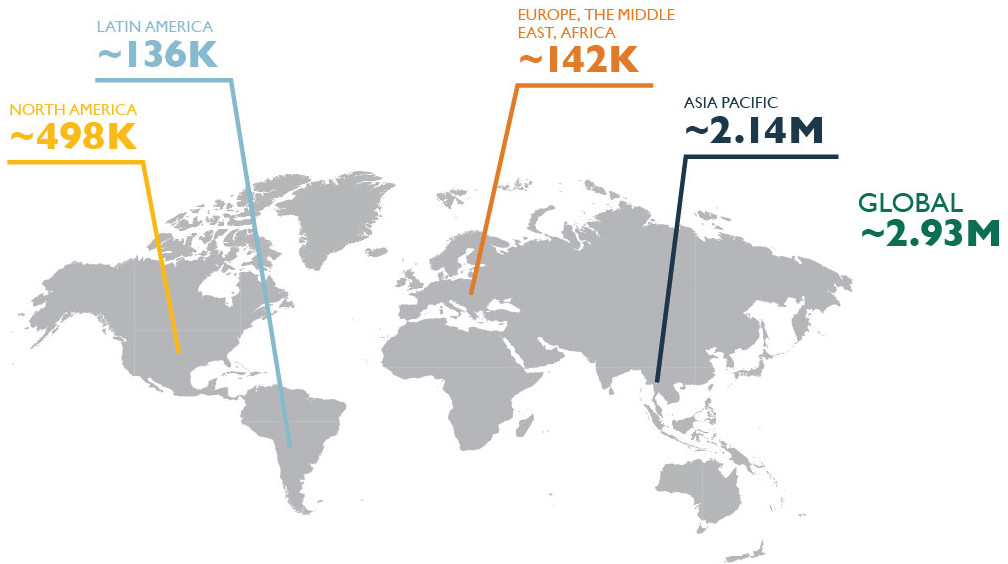
\includegraphics[width=0.8\linewidth]{figures/introduction/expertise.jpg}}
        \caption[Cybersecurity skills shortage around the globe]{Cybersecurity skills shortage around the globe, (ISC)$^2$ Cybersecurity Workforce Study~\cite{ics2_cybersecurity_2018}}
	\label{figure:introduction:expertise}
\end{figure}

The use of automation techniques by security attackers also worsens the situation.
Every day, AV-Test registers over 350,000 new malicious programs and potentially unwanted applications across all computer platforms~\cite{av-test_malware_2019}.
On Figure~\ref{figure:introduction:profusion}, we track the development of new Android malware over the years.
While only a few samples were registered in 2012, the number of malware accelerated and peaked in 2016 and 2017 with more than 4 million malware every year.
In 2018, six new Android malware were created every minute.
We can conclude from these figures that the sheer amount of malware created in the world must be generated automatically by computer systems.

\begin{figure}[!ht]
        \centering
	\fbox{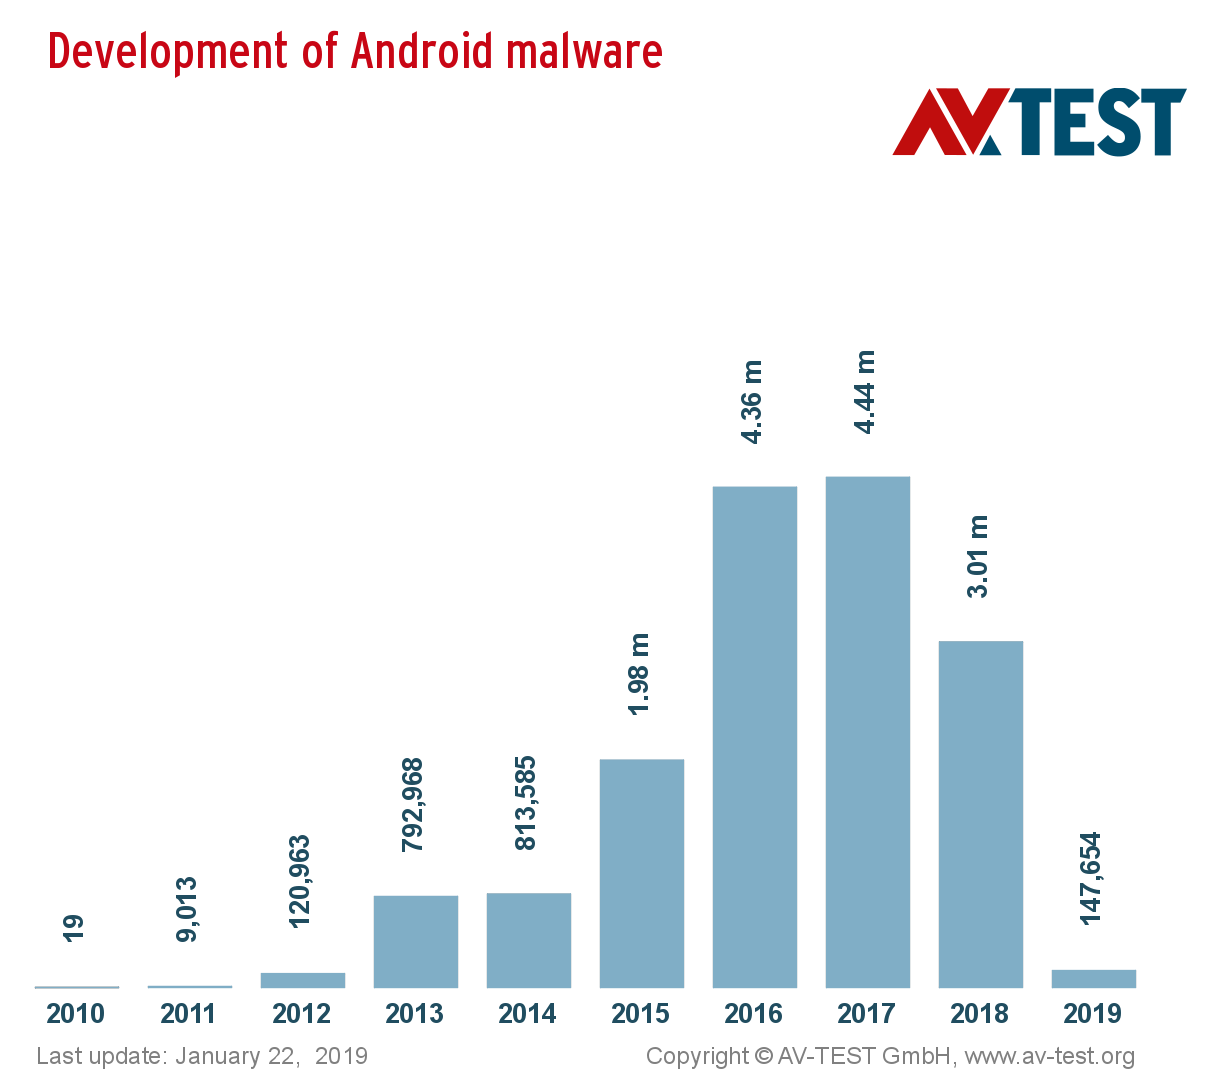
\includegraphics[width=0.75\linewidth]{figures/introduction/profusion.png}}
        \caption[Registration of new Android malware over the years]{Registration of new Android malware over the years, AV-Test~\cite{av-test_malware_2019}}
	\label{figure:introduction:profusion}
\end{figure}

To answer both the lack of security experts and the velocity of malware proliferation, organizations are actively seeking alternative solutions.
In 2018, Forbes mentioned that new technology such as big data, artificial intelligence, and machine learning have the potential to address the lack of human resources~\cite{forbes_cybersecurity_2018}.
Furthermore, security solutions could also improve the security of our infrastructures, as computers are capable of handling billions of security events per hour while humans can only process a limited amount of events and during a short period.
For these reasons, the creation of human-aided assistants is an crucial objective for the field of Android security and the security of information systems in general.
\subsubsection{Machine learning to the rescue}
As a substitute for human resources, the security community has turned its attention to a branch of artificial intelligence called machine learning.
In essence, machine learning is the application of algorithms and statistics to train computer systems in performing a specific task.
For instance, machine learning is commonly used on Android devices to translate speech to text, recognize digital prints, or adjust energy consumption based on user preferences.
Machine learning algorithms excel in situations where data is abundant and well-annotated.
In this case, experts can rely on supervised learning, a subset of machine learning focused on training computer systems based on real-world examples.

Figure~\ref{figure:introduction:learning} illustrates the components involved during the training of supervised learning systems.
From raw input data, the algorithm progressively tunes a statistical model based on a training set and an output selected by a human supervisor.
For instance, if the task of the algorithm is to predict a type of fruit, then the model can rely on previous examples to make prediction for unknown cases.
The learning process of the algorithm is similar to the sequence of steps followed by a human student.
In both cases, the student and the algorithm take into account feedbacks that encourages them to change their decision when they make a mistake.
On the contrary, the right decision will strengthen the current model and improve their confidence.
To verify that the training is complete, model predictions are then compared against a testing set that was left out from the initial dataset.
The training and testing sets constitute the ground truth and are used by machine learning practitioners during their experiments.
It is important to note that human supervision remains crucial to train supervised learning algorithms, as the choice of inputs and outputs originates from a human operator.

\begin{figure}[!ht]
        \centering
	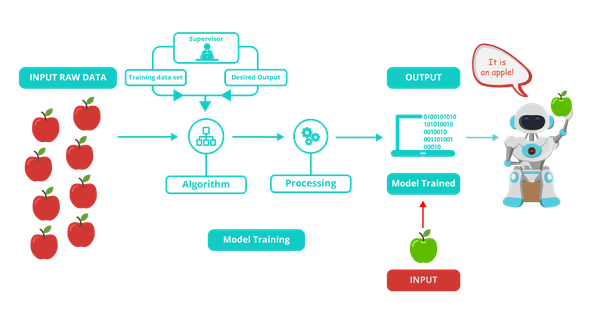
\includegraphics[width=\linewidth]{figures/introduction/supervised.png}
        \caption[Supervised learning is the process of learning from annotated examples]{Supervised learning is the process of learning from annotated examples~\cite{vaseekaran_machine_2018}}
	\label{figure:introduction:learning}
\end{figure}

While machine learning algorithms have greatly improved our capacity to automate security decisions, their performance depends heavily on the quality of the ground truth chosen during the training and verification of statistical models.
The problem of ground truth quality is recurrent, and often referred in computer science by the term `Garbage in, garbage out', which implies that flawed input data produces flawed output data.
In the absence of qualified ground truth datasets, machine learning techniques cannot be trusted to analyze Android malware in production, as their predictions might introduce both false positive and false negative detections.
\subsection{Progression of human comprehension}
\subsubsection{The curse of dimensionality}
Despite the recent use of machine learning, digital marketplaces are not in a position to fully automate the detection of Android malware.
As we reviewed in the last section, machine learning algorithms require a large set of well-annotated malware samples that only human experts can provide.
While unsupervised learning techniques can be applied to collect more annotation, the analysis of a single malware is a time-consuming task that incurs a bottleneck in the annotation process.

The situation faced by security experts is similar to a phenomenon observed in computer science called the curse of dimensionality~\cite{bellman_dynamic_2013}.
As the number of items to look at (a.k.a, dimensions) increases, the sparsity and the complexity of data inflates to a point where both the analysis and the prediction become much less efficient.
Android applications are complex pieces of software that share the same property.
Figure~\ref{figure:introduction:complexity} shows the distribution of Android applications size collected by the Androzoo project~\cite{allix_androzoo:_2016}, as a proxy measure to analyze their complexity.
We notice that both plots follow a power law distribution, with an average source code size of 3.5 MB and an average application size of 10.4 MB.
Csikszentmihalyi et al.~\cite{csikszentmihalyi_flow_2014} found that a human can only process 15 bytes per second.
Thus, we can compute that it would take about 68 hours to process the information contained in the source code alone and 202 hours to look at the whole Android application.

\begin{figure}[!ht]
        \centering
	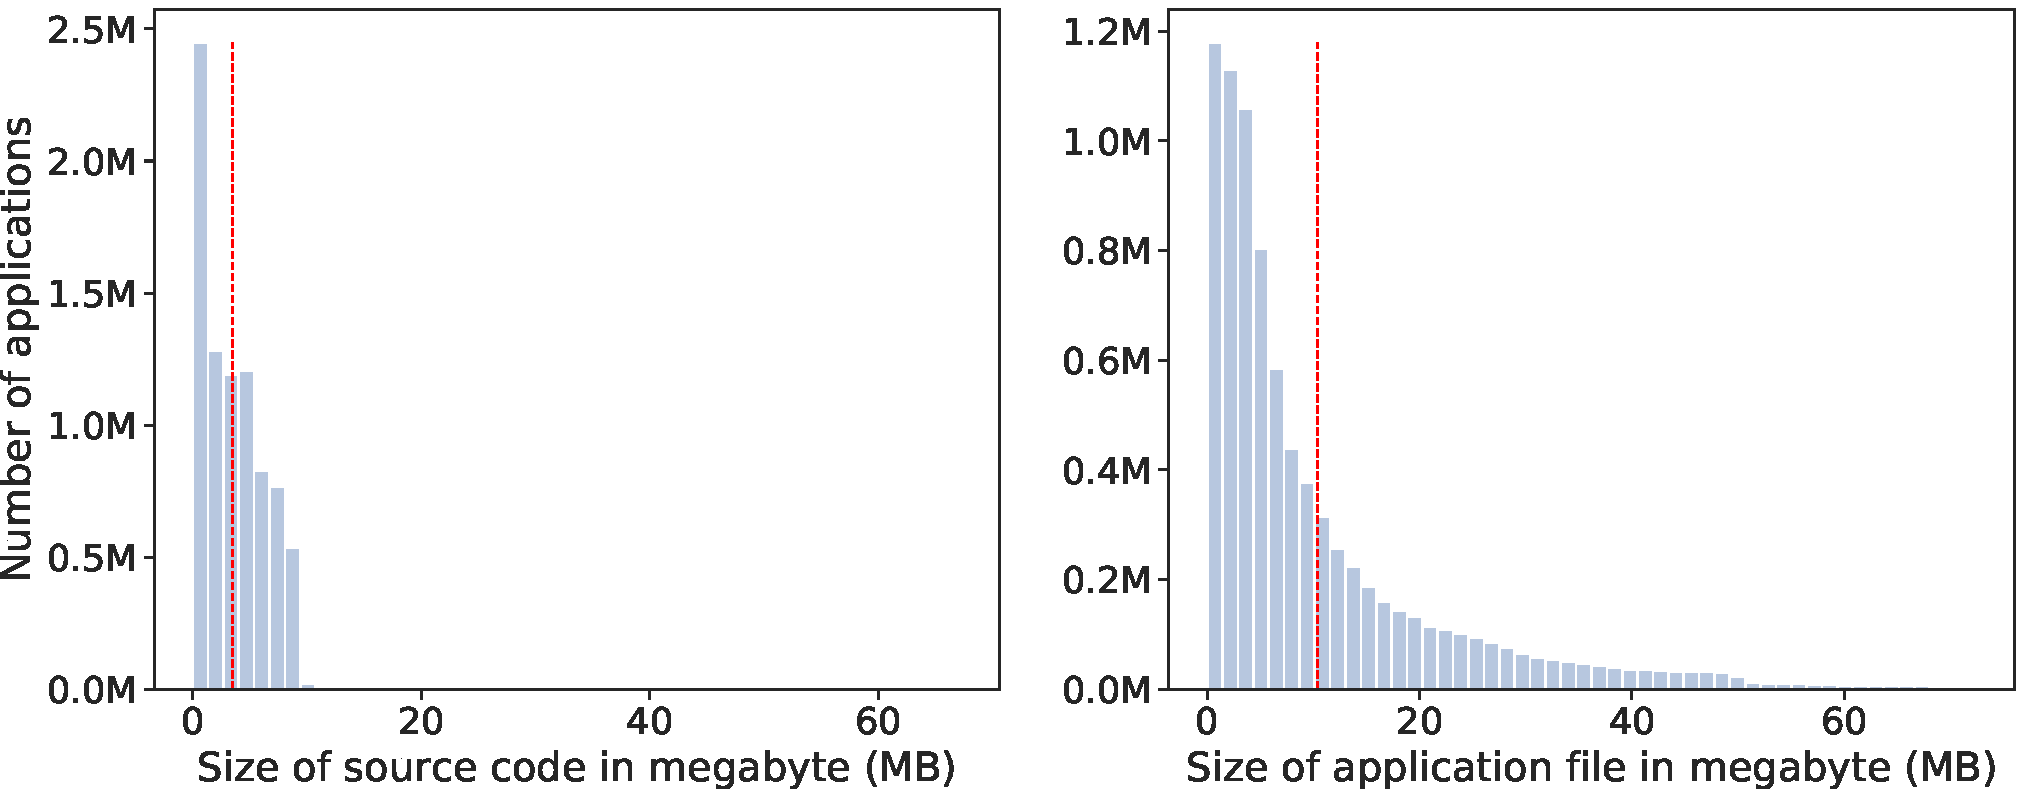
\includegraphics[width=\linewidth]{figures/introduction/complexity.pdf}
	\caption{Complexity metrics of Android applications found on Androzoo}
	\label{figure:introduction:complexity}
\end{figure}

As our protection solutions continue to mature, the security community must propose new ways to improve the processing capacity of human analysts.
Since we can not increase the bandwidth of the human brain, our technology must compensate for our lack of analysis power by providing a smarter output and by focusing our attention on the details that matter.
This condition is critical both to augment our protection mechanisms against malware and to become more efficient at detecting new malware threats.
\subsubsection{Dissection of Android malware}
To understand the behaviors of Android malware, security analysts have no choice but to inspect the components of Android applications one after the other.
This operation, called reverse engineering, is similar for all intents and purposes to the dissection of a living organism.
The goal of a reverse engineer is to start with a final product, and then retrieve the source code of the application.
At the end of the analysis, human experts try to answer a few basic questions about the malware:

\begin{itemize}
	\item What does the application do?
	\item Who is the author of the application?
	\item Which of its components are malicious?
	\item Where are malicious components located?
	\item Which other applications include its components?
\end{itemize}

The data required to answer these questions can take hours, and even days to gather, even for a small application.
For instance, Figure~\ref{figure:introduction:dissection} shows the elements scrutinized by security analysts to understand the behavior of Android applications.
In addition to the application source code, security analysts must look at the files, assets, services, and messages contained in the application.
Moreover, malware authors attempt to hide the true nature of their application by using obfuscation techniques.
This scheme prevents security analysts from reading the resources directly, which slows down the analysis even more.

\begin{figure}[!ht]
	\centering
	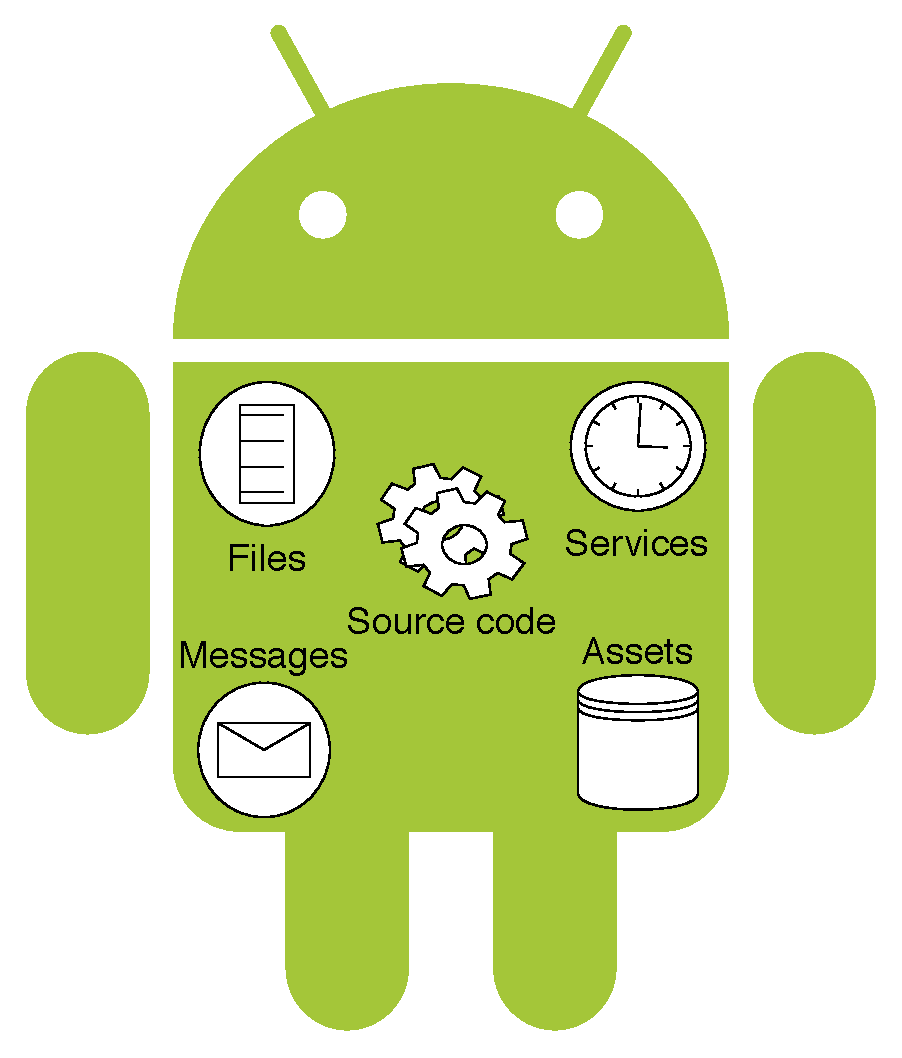
\includegraphics[width=0.45\linewidth]{figures/introduction/dissection.pdf}
	\caption{Artifacts that can be extracted from an Android application}
	\label{figure:introduction:dissection}
\end{figure}

A computer system capable of answering these questions would be a valuable asset for a security analyst.
Not only could the system speed up the analysis process, but it could also establish the foundation for a knowledge base about Android malware and serve the whole security community.
The main challenge imposed on the dissection of Android malware is to provide an approach capable of handling a vast amount of data at scale.
\section{Contributions to the realm of Android security}
\subsection{Qualification of malware datasets}
\subsubsection{Metrics to understand malware datasets}
As we have seen in the previous section, the performance of machine learning based systems depends heavily on the quality of the samples chosen to support the learning process.
This requirement means that the security community must have access to large sets of qualified Android applications to detect and classify various kinds of malware.
However, the analysis of Android malware remains tedious and time consuming for security experts.

Different approaches have been proposed to create malware datasets based on samples found in the wild, each with their advantages, drawbacks, and biases.
A standard method for machine learning practitioners is to rely on external labeling services such as VirusTotal~\cite{noauthor_virustotal_nodate} to alleviate the need for analyzing Android application manually~\cite{arp_drebin:_2014}.
Alternatively, other research groups worked with established malware datasets~\cite{zhou_dissecting_2012}, as these sets are both well-studied and readily available to the community.
In either case, the research community must consider the impact that these choices have on their datasets.

\begin{mdframed}[hidealllines=true,nobreak=true]
\textbf{Questions:}

\begin{enumerate}
	\item What are the impacts of malware ground truth used in research experiments?
	\item How do malware datasets compare with each other, and what are their desirable properties?
	\item Do malware datasets incorporate biases due to their creation method or to their origin?
\end{enumerate}
\end{mdframed}

To answer these questions, Chapter~\ref{chapter:stase} introduces STASE, a framework created to measure the characteristics of malware datasets.
Based on a set of 9 metrics, STASE highlights the key properties of malware ground truth employed either to detect malware or classify applications in different threat groups.
For instance, STASE can measure the degree of consensus across antivirus products or inform about the degree of confidence that a particular application is indeed malicious.
The practical goal of STASE is to provide an overview of the features entrenched in malware ground truth before their use in research experiments.
STASE metrics can also report information a posteriori to scrutinize biases in malware datasets and assess that the properties of ground truth are comparable to previous studies.

\begin{mdframed}[hidealllines=true,nobreak=true]
\textbf{Contributions}:

\begin{enumerate}
	\item We define a set of nine metrics that quantifies the main characteristics of malware datasets created from the aggregation of antivirus results.
	\item We provide a framework to encourage the development of heuristics that increases the confidence in malware dataset by removing potential biases.
	\item We propose a method to compare malware datasets against each other and ensure that the properties of malware ground truth remain faithful over time.
\end{enumerate}
\end{mdframed}

\subsubsection{Evaluation of common malware datasets}
Over the past few years, the research community around Android security has adopted two popular malware datasets for their experiments.
The first dataset was assembled under the umbrella of the Android Malware Genome Project by the North Carolina State University between 2010 and 2011~\cite{zhou_dissecting_2012}.
MalGenome includes 1,200 malicious applications and covers popular Android malware families found at the time of the study.
The specificity of this dataset is that most samples were analyzed manually by a team of students.
Thus, many aspects of the applications, including the installation method, the activation mechanisms, and the nature of the malware payload, have been inspected and studied by the Android community.
The other popular malware dataset was created by the Technische Universität Braunschweig between 2010 and 2012 under the name Drebin.
Compared to MalGenome, this dataset was analyzed with a mix of both manual and automated techniques.
The authors of Drebin mention that their dataset contains 5,560 applications divided into 179 malware families.
With various datasets at their disposal, the security community has to design experiments with the most representative samples that represent the whole population of Android malware.

\begin{mdframed}[hidealllines=true,nobreak=true]
\textbf{Questions:}

\begin{enumerate}
	\item How are the properties of common malware datasets influenced by the methodology used to construct these sets?
	\item Do the degree of confidence and the degree of consensus in the dataset vary according to the choice of malware construction techniques?
	\item What are the distinctions between well-known malware datasets and recent malware samples collected directly from the Internet?
\end{enumerate}
\end{mdframed}

With the help of STASE, Chapter~\ref{chapter:stase} presents an empirical study on the most common techniques used to build ground truths of Android malware.
In the first part, our study reviews the capacity of antivirus systems to decide if an Android application is malicious or not.
In the second part, our study analyzes the quality of the information mentioned in the label returned by antivirus systems.
Our evaluation reveals that the degree of consensus between antivirus is often low and that some antiviruses provide fairly generic labels.
Moreover, the selection of antivirus systems has a significant influence on the characteristics of the dataset, such as the ability to divide malware into unambiguous threat groups.
Thus, machine learning practitioners are encouraged to pick the subset of antivirus systems that provides either the highest degree of confidence or the largest amount of information depending on their use cases.

\begin{mdframed}[hidealllines=true,nobreak=true]
\textbf{Contributions:}

\begin{enumerate}
	\item We review the difference between popular malware datasets according to STASE in order to quantify the disparity between common dataset construction techniques.
	\item We provide insights on the practice of building ground truth datasets based on VirusTotal labeling service and a large dataset of thousands of Android applications.
	\item We extensively overview the lack of consensus between both antivirus decisions and antivirus labels to call for new approaches in building authoritative malware ground truth.
\end{enumerate}
\end{mdframed}

\subsection{Unification of malware information}
\subsubsection{Extraction from malware labels}
To conduct experiments on Android malware, we mentioned that the security community depends either on well-studied malware sets or Android applications amassed directly from the Internet.
While the former method has the benefit of leveraging knowledge from previous works, the latter method provides larger datasets and a more up to date view of the current malware landscape.
To illustrate this difference, let us consider the AndroZoo project, which provides Android applications downloaded from official and third-party markets to the research community~\cite{allix_androzoo:_2016}.
As of January 2019, the project references more than 8 million applications compiled from 2008 to 2019.
Compared to well-studied datasets such as Drebin~\cite{arp_drebin:_2014} or MalGenome~\cite{zhou_dissecting_2012}, Androzoo contains 1,500 times more samples and over a period of time nine years larger.
However, the idea of using samples collected in the wild has a major setback.
Without proper information about the true nature of applications gathered with this method, experimenters are not in possession of a ground truth that enables them to decide which applications should be considered malicious.

To address the lack of information about Android malware, the security community must rely on external sources of information to review the content of Android applications.
The solution currently favored by the security community is VirusTotal~\cite{noauthor_virustotal_nodate}, an online service that acts as a proxy to antivirus solutions available to the security industry.
Once an Android application is submitted to VirusTotal, a set of antivirus analyzes the application and returns their decision in the form of a malware label (i.e.,\ a string of characters that embedded several information about the applications).
For example, Figure~\ref{figure:introduction:label} shows a single malware label that contains four parts: the threat type (monitoring tool), the platform (Android), family name (AccuTrack) and the variant (Beta).
However, while labels information is intelligible to human experts, their interpretation by computer systems is a challenging task.
On the one hand, the syntax of labels (i.e.,\ the position and separation of information tokens) varies across antivirus solutions and sometimes even inside a single antivirus product.
On the other hand, the semantic (i.e.,\ the vocabulary and lexicon) is not stable as different labels can be assigned to the same underlying threat.

\begin{figure}[!ht]
        \centering
	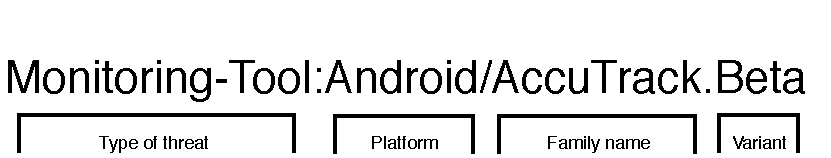
\includegraphics[width=0.75\linewidth]{figures/introduction/label.pdf}
        \caption[Example of an antivirus label reported by VirusTotal]{Example of an antivirus label reported by VirusTotal (with information annotated)}
	\label{figure:introduction:label}
\end{figure}

\begin{mdframed}[hidealllines=true,nobreak=true]
\textbf{Questions:}

\begin{enumerate}
	\item How to accurately extract the information contained in antivirus labels?
	\item Can the process of extracting information from antivirus label be automated?
	\item What is the minimum amount of knowledge required to extract label information?
\end{enumerate}
\end{mdframed}

To address these challenges, we introduce EUPHONY in Chapter~\ref{chapter:euphony}.
EUPHONY is a heuristics and statistics based system that extracts information from malware labels.
Compared to previous solutions, the distinctive feature of EUPHONY is its ability to improve its extraction performance over time, starting from a minimal vocabulary up to much larger lexicons.
This feature is critical for the discovery of new threats, as more and more types of malicious techniques are uncovered and identified over time.
In practice, we expect EUPHONY to be used both by industrial and academic actors willing to automate the recovery of information from malware labels.
Finally, the performance of EUPHONY has been successfully tested both on well-known malware datasets and on the Androzoo project to propose a larger ground truth of Android applications.

\begin{mdframed}[hidealllines=true,nobreak=true]
\textbf{Contributions:}

\begin{enumerate}
	\item We present the design and implementation of EUPHONY, an approach designed to mine the information contained in antivirus labels gathered from malware samples found in the wild.
	\item We report the evaluation of EUPHONY on MalGenome~\cite{zhou_dissecting_2012} and Drebin~\cite{arp_drebin:_2014} datasets, where EUPHONY achieves relatively high performance of 92.7\% and 95.5\% F-measure respectively.
	\item We examine the distinctive features of EUPHONY in contrast with previous work, such as the ability to automatically learn the structure and lexicon of antivirus labels and to iteratively improve the inference performance over time.
\end{enumerate}
\end{mdframed}

\subsubsection{Aggregation of malware families}
Out of the different label parts, the most valuable element is the family name associated with the malware, as this name identifies a particular type of threat that shares common attributes with other members of its family.
For instance, the AccuTrack family is known to turn Android smartphones into GPS trackers and display unwanted ads to the device owner~\cite{solvusoft_how_nodate}.
This knowledge could be leveraged to focus the attention of security experts on the application components responsible for user geolocation.

However, the extraction process of EUPHONY only addresses the surface of the problem, which is to remove the elements of syntax specific to each antivirus system.
The lack of naming convention potentially implies that antivirus systems do not share the same semantic, and that different family names could reference the same applications.
In this situation, security experts could not distinguish between a problem of consensus between antivirus systems and a case where two family names are aliases of each other.
To prevent this issue, the security community must have a solution that proposes a single malware name for each sample present in a set of applications, even if they are classified by multiple antivirus systems that follow different conventions.

\begin{mdframed}[hidealllines=true,nobreak=true]
\textbf{Questions:}

\begin{enumerate}
	\item How can we evaluate the similarity between antivirus labels?
	\item At which conditions can malware names be unified into a single name?
	\item How can we apply a unification scheme to malicious applications found in the wild?
\end{enumerate}
\end{mdframed}

To address these issues, EUPHONY provides a module that clusters family names into cohesive groups.
The primary purpose of the clustering module is to aggregate malware families when their names appear jointly on the same set of applications.
Based on these observations, EUPHONY can model the association between family names in the form of a weighted graph and find substructures that maximize the strength of their relationship.
On the contrary, relationships between family names that are too weak are removed to create new family names.
The clustering module allows malware practitioners to obtain a single family name per application, even if they rely on multiple antiviruses to improve their confidence in antivirus decisions.
With this technique, EUPHONY can create malware ground truths that combine samples collected in the wild and antivirus reports gathered with VirusTotal.

\begin{mdframed}[hidealllines=true,nobreak=true]
\textbf{Contributions:}

\begin{enumerate}
	\item We propose a clustering scheme as part of EUPHONY that infers the family names of malicious applications based on their co-occurrence in malware datasets.
        \item We provide the security community with a new and larger dataset of Android malware constructed from the annotation inferred by EUPHONY for the Androzoo project~\cite{allix_androzoo:_2016}.
	\item We release EUPHONY as an open source application to support the creation of better malware ground truth based on antivirus reports gathered from VirusTotal.
\end{enumerate}
\end{mdframed}

\subsection{Dissection of malicious components}
\subsubsection{Gathering knowledge on malware}
We observed in the previous section that the protection mechanisms of our infrastructure are centered around two activities: the deployment of detection systems in production and the collection of knowledge to improve the performance of these systems.
The compilation of knowledge is a fundamental aspect to the security community, as the pertinence of statistical models fades as soon as malware authors turn their attention to new pervasion techniques.
Thus, the constant pace of modification required to update systems in production depends on our capacity to mine Android malware as fast as malicious applications are released to the world.
However, the dissection of malicious applications is not in a satisfying state of automation.
Firstly, malware dissection is performed by human experts and requires hours and sometimes days to reverse even a single malicious application.
Secondly, navigating the vast amount of components found in Android applications is a slow process, as humans are not accustomed to work at this level of complexity.

To improve the dissection of Android applications, security experts must have access to a database dedicated to the collection of knowledge about malware.
This knowledge base would be a valuable asset, as it could be queried to reveal the relationship between Android applications and the internal components linked to the expression of malicious behaviors.
The database could also work as a hub that stores various kind of metadata gathered from Android malware analysis.
With this system in place, practitioners could work at a higher level of understanding and craft new features with a more comprehensive process.
However, as the number of components found in Android applications is likely huge, the security community must deal with several challenges.

\begin{mdframed}[hidealllines=true,nobreak=true]
\textbf{Questions:}

\begin{enumerate}
	\item How to represent the association between Android applications and malicious artifacts?
	\item What kind of information is essential to analyze the behavior of Android applications?
	\item Which techniques can be applied to limit the lack of scalability of knowledge indexing?
\end{enumerate}
\end{mdframed}

In Chapter~\ref{chapter:apgraph}, we introduce AP-GRAPH as a knowledge base designed to store and extract information from large sets of Android applications.
The model of AP-GRAPH is focused on exploring the relationship between applications and their internal components, also called artifacts.
Both applications and artifacts are represented as nodes in a graph, linked together by edges to express the relationship between them.
The main benefit of AP-GRAPH is to provide a database that supports a wide range of query, opening to a new way of looking at Android applications.
AP-GRAPH can be used by security experts to find applications impacted by particular malicious artifacts or to uncovered potentially harmful artifacts based on analytic queries.

\begin{mdframed}[hidealllines=true,nobreak=true]
\textbf{Contributions:}

\begin{enumerate}
	\item We propose a representation model for exploring the relationship between Android applications and artifacts that are potentially harmful.
	\item We postulate that the knowledge provided by AP-GRAPH can improve our understanding of malicious applications by providing a graph structure focused on the relationship between applications and artifacts.
	\item We publish an online service named APKSEARCH to let other researchers query the associations uncovered by AP-GRAPH and let them create more relevant training sets for their experiments.
\end{enumerate}
\end{mdframed}

\subsubsection{Locating potentially malicious artifacts}
To automate the dissection of Android malware, we postulate that malicious behaviors associated with malware are linked to at least one internal component of the application.
For instance, a fake banking application that steals personal information cloud include a service that collects data in the background or an activity that gives the impression that the application is benign.
Even if malicious components could be first downloaded from the Internet, there must be a part of the application responsible for downloading and executing the remote code.
Hence, the presence of artifacts within Android applications could be exploited by computer systems to draw associations between malware files and malicious behaviors.

With the information produced by both EUPHONY and AP-GRAPH, we have access respectively to information about malicious behaviors linked to family names and artifacts related to Android applications.
Thus, large sets of Android malware gathered by the security community could be mined to locate suspicious elements in place of security experts.
The gain for the security community would be enormous, as security experts allocate a considerable amount of time on the location of relevant pieces of information within Android applications.
The feasibility of this approach would depend on several criteria:

\begin{mdframed}[hidealllines=true,nobreak=true]
\textbf{Questions:}

\begin{enumerate}
	\item How can we determine that an artifact is related to the malicious behavior of an application?
	\item At which point can we consider that a malicious artifact is tied precisely to a malware family?
	\item Which method can be used to find the location a malicious artifact once revealed by an automated approach?
\end{enumerate}
\end{mdframed}

Chapter~\ref{chapter:apgraph} presents how AP-GRAPH database can be applied to locate potentially malicious artifacts.
Using the occurrence of artifacts within malware families, AP-GRAPH can filter the most relevant artifacts and report components specific to a malware family.
Moreover, AP-GRAPH could be used to maintain both a white list of artifacts found in benign applications and a black list of artifacts that should trigger a security alarm.
Thus, the approach we propose could assist security experts in finding both known and unknown malicious artifacts.
Applied to a large set of malware such as Androzoo~\cite{allix_androzoo:_2016}, AP-GRAPH could support the creation of a malware a ground truth composed of artifacts strongly correlated with malicious behaviors.

\begin{mdframed}[hidealllines=true,nobreak=true]
\textbf{Contributions:}

\begin{enumerate}
	\item We propose a scheme to automatically locate potentially malicious artifacts that are associated with malware families extracted from antivirus solutions.
	\item We perform a systematic study on the most important Android malware families collected by the research community. In particular, we explain that thousands of malware artifacts are directly linked to specific malware families.
	\item We release a public dataset of malware descriptions mined by AP-GRAPH to support the continuous effort of the research community in preventing the propagation of malicious applications.
\end{enumerate}
\end{mdframed}
